\documentclass[aspectratio=169]{beamer}
\usepackage{will_handley_beamer}
\usepackage{title_page}

% Commands
% --------
% - \arxiv{arxiv number}
% - \arxiv{<number>}            arxiv.org/abs/<number>
% - \oldarxiv{<arxiv number>}   arxiv.org/<number>
% - \doi{<doi>}                 doi.org/<doi>
% - \xkcd{<number>}             xkcd.com/<number>
% - \email{<email>}             <<email>>
% - \tthref{<website>}          <website>
% - \av[dist]{<quantity>}       <quantity>_{dist}
% - \student{<name>}{<detail>}{<photo>}

% Talk details
% ------------
\title{GPU-native nested sampling in BlackJAX}
\subtitle{Accelerating Bayesian inference to state-of-the-art levels}
\date{<+Date+>}

\begin{document}

\begin{frame}
    \titlepage
\end{frame}

\begin{frame}
    \frametitle{Astrostatistics: Real-Time Inference for Gravitational Wave Astronomy}
    \begin{columns}
        \column{0.48\textwidth}
        \begin{block}{The Challenge: GW170817}
            \begin{itemize}
                \item \textbf{Gravitational wave detected}: Binary neutron star merger
                \item \textbf{Real-time parameter estimation}: 15+ dimensional space
                \item \textbf{Sky localization}: $\sim 30$ square degrees uncertainty
                \item \textbf{EM counterpart follow-up}: Telescopes need targets within hours
            \end{itemize}
        \end{block}
        \begin{block}{Statistical Requirements}
            \begin{itemize}
                \item \textbf{Parameter estimation}: Masses, spins, distance, sky position
                \item \textbf{Model comparison}: Signal vs noise, waveform models
                \item \textbf{Uncertainty quantification}: Posterior credible regions
                \item \textbf{Speed}: Results needed for telescope scheduling
            \end{itemize}
        \end{block}
        \column{0.48\textwidth}
        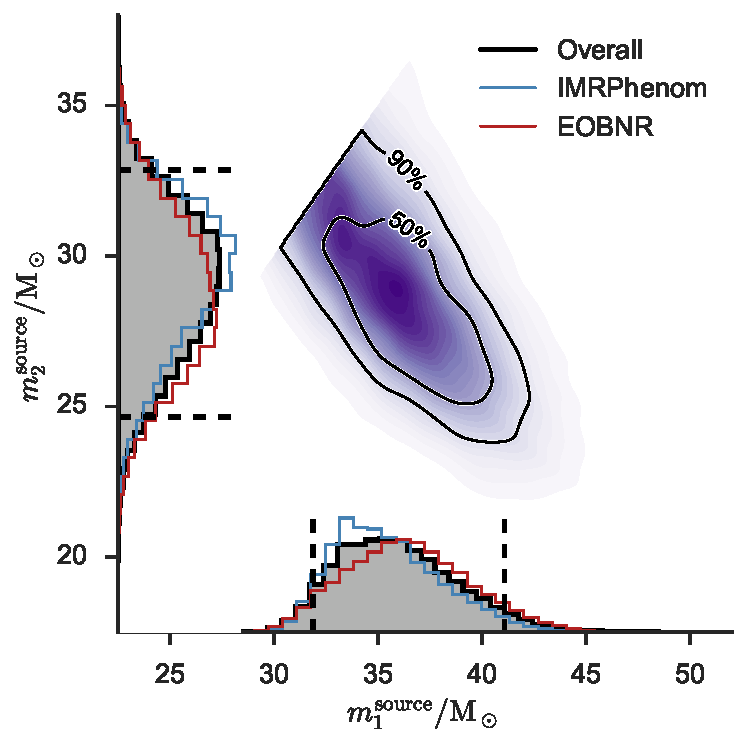
\includegraphics[width=0.49\textwidth]{figures/ligo_m1_m2}
        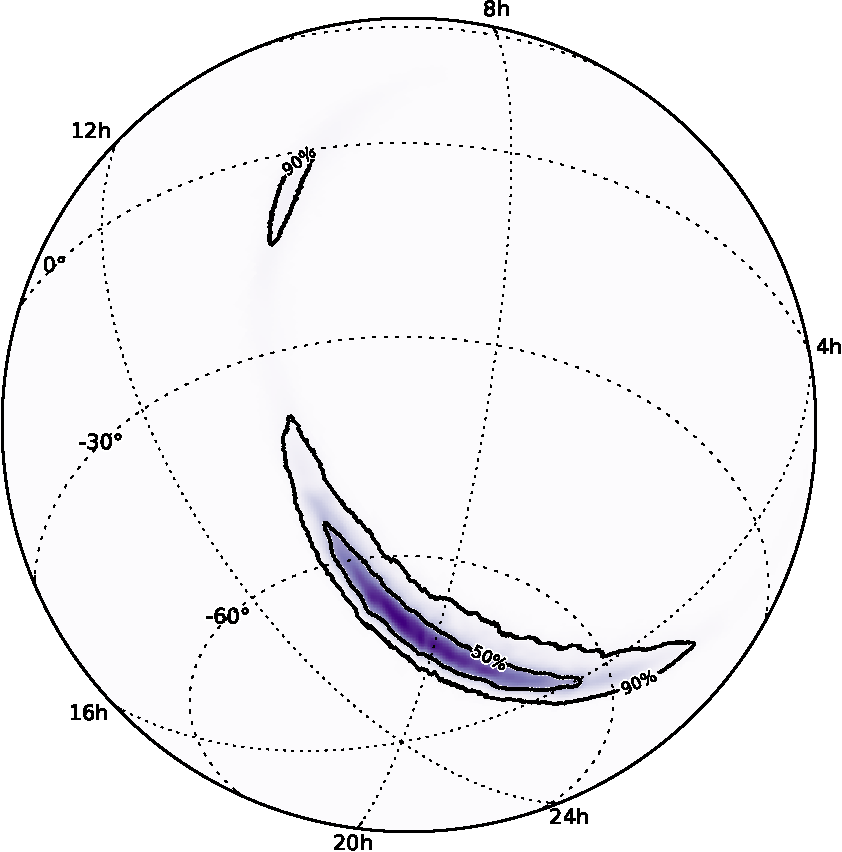
\includegraphics[width=0.49\textwidth]{figures/ligo_lambert-skymap}
        \vspace{10pt}
        \begin{block}{The Broader Astrostatistics Context}
            \begin{itemize}
                \item \textbf{High-dimensional}: $d \sim 10^2$--$10^3$ parameters
                \item \textbf{Multimodal}: Competing physical models
                \item \textbf{Expensive likelihoods}: Complex simulations
                \item \textbf{Model selection critical}: Which physics to include?
            \end{itemize}
        \end{block}
    \end{columns}
\end{frame}

\begin{frame}
    \frametitle{The Bayesian Inference Challenge}
    \begin{columns}
        \column{0.48\textwidth}
        \begin{block}{Parameter Estimation}
            \begin{itemize}
                \item Posterior: $p(\theta|D) \propto \mathcal{L}(D|\theta) \pi(\theta)$
                \item Need samples from $p(\theta|D)$
                \item Standard approach: MCMC methods
                \item Well-solved problem in many cases
            \end{itemize}
        \end{block}
        \begin{block}{Model Comparison}
            \begin{itemize}
                \item Evidence: $\mathcal{Z} = \int \mathcal{L}(D|\theta) \pi(\theta) d\theta$
                \item Bayes factors: $\mathcal{B}_{12} = \mathcal{Z}_1 / \mathcal{Z}_2$
                \item \textbf{Much harder problem}
                \item MCMC doesn't estimate $\mathcal{Z}$ directly
            \end{itemize}
        \end{block}
        \column{0.48\textwidth}
        \begin{block}{Challenges for Modern Science}
            \begin{itemize}
                \item \textbf{High dimensions}: $d \sim 10^2$--$10^3$
                \item \textbf{Multimodality}: Multiple competing theories
                \item \textbf{Computational cost}: Complex forward models
                \item \textbf{Model selection}: Which physics to include?
            \end{itemize}
        \end{block}
        \vspace{10pt}
        \begin{center}
            \textbf{Key Insight:}\\
            Need methods that compute \emph{both} \\
            posterior samples \emph{and} evidence
        \end{center}
    \end{columns}
\end{frame}

\begin{frame}
    \frametitle{Sampling Methods for Bayesian Inference}
    \begin{columns}
        \column{0.5\textwidth}
        \begin{block}{Single-Chain MCMC}
            \begin{itemize}
                \item \textbf{Metropolis-Hastings}: Simple, widely used (PyMC)
                \item \textbf{HMC/NUTS}: Gradient-based, efficient (Stan, BlackJAX)
                \item \textbf{Strengths}: Fast for unimodal, well-conditioned problems
                \item \textbf{Limitations}: Poor multimodal mixing, no evidence
            \end{itemize}
        \end{block}
        \begin{block}{Ensemble Methods}
            \begin{itemize}
                \item \textbf{Affine-invariant}: emcee, zeus - excellent multimodal sampling
                \item \textbf{Sequential Monte Carlo}: Tempering, annealing
                \item \textbf{Nested Sampling}: Evidence-focused, robust multimodal
                \item \textbf{Strengths}: Handle multimodality, some estimate evidence
                \item \textbf{GPU Advantage}: Natural vectorization across ensemble
            \end{itemize}
        \end{block}
        \column{0.5\textwidth}
        \begin{columns}
            \column{0.5\textwidth}
        \includegraphics[width=\textwidth]{figures/emcee}
        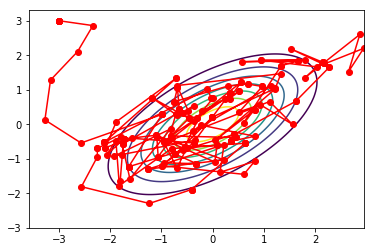
\includegraphics[width=\textwidth]{figures/metropolis-hastings}
            \column{0.5\textwidth}
        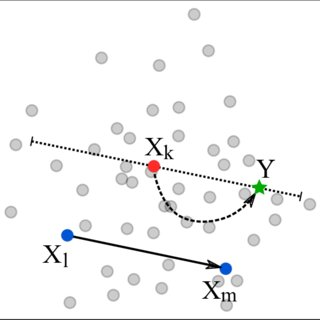
\includegraphics[width=\textwidth]{figures/zeus}
        \end{columns}
        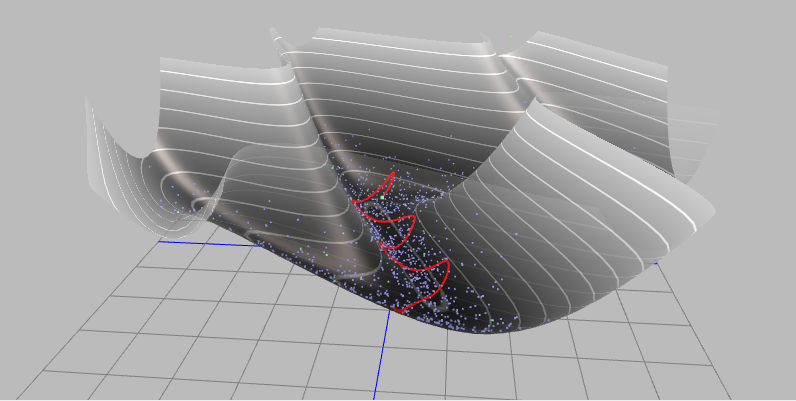
\includegraphics[width=\textwidth]{figures/hmc_explained}
        \vspace{5pt}
        \begin{center}
            \textbf{Nested sampling}: \\
            Unique in targeting \\
            evidence computation directly
        \end{center}
    \end{columns}
\end{frame}

\begin{frame}
    \begin{columns}
        \column{0.48\textwidth}
        \begin{block}{\textbf{MCMC}}
            \only<16>{
                \begin{itemize}
                    \item Single ``walker''
                    \item Explores posterior
                    \item Fast, if proposal matrix is tuned
                    \item Parameter estimation, suspiciousness calculation
                    \item Channel capacity optimised for generating posterior samples
                \end{itemize}
            }
        \end{block}
            \includegraphics<1>[width=\textwidth,page=1]{figures/himmelblau_mcmc}%
            \includegraphics<2>[width=\textwidth,page=2]{figures/himmelblau_mcmc}%
            \includegraphics<3>[width=\textwidth,page=3]{figures/himmelblau_mcmc}%
            \includegraphics<4>[width=\textwidth,page=4]{figures/himmelblau_mcmc}%
            \includegraphics<5>[width=\textwidth,page=5]{figures/himmelblau_mcmc}%
            \includegraphics<6-15>[width=\textwidth,page=9]{figures/himmelblau_mcmc}%
        \centerline{\includegraphics<16>[width=0.5\textwidth,page=9]{figures/himmelblau_mcmc}}
        \column{0.48\textwidth}
        \begin{block}<7->{\textbf{Nested sampling}}
            \only<16>{
                \begin{itemize}
                    \item Ensemble of ``live points''
                    \item Scans from prior to peak of likelihood
                    \item Slower, no tuning required
                    \item Parameter estimation, model comparison, tension quantification
                    \item Channel capacity optimised for computing partition function
                \end{itemize}
            }
        \end{block}
            \includegraphics<7|handout:0>[width=\textwidth,page=1]{figures/himmelblau_ns}%
            \includegraphics<8|handout:0>[width=\textwidth,page=2]{figures/himmelblau_ns}%
            \includegraphics<9|handout:0>[width=\textwidth,page=3]{figures/himmelblau_ns}%
            \includegraphics<10          >[width=\textwidth,page=4]{figures/himmelblau_ns}%
            \includegraphics<11|handout:0>[width=\textwidth,page=5]{figures/himmelblau_ns}%
            \includegraphics<12|handout:0>[width=\textwidth,page=6]{figures/himmelblau_ns}%
            \includegraphics<13|handout:0>[width=\textwidth,page=7]{figures/himmelblau_ns}%
            \includegraphics<14|handout:0>[width=\textwidth,page=8]{figures/himmelblau_ns}%
            \includegraphics<15|handout:0>[width=\textwidth,page=8]{figures/himmelblau_ns}%
        \centerline{\includegraphics<16>[width=0.5\textwidth,page=4]{figures/himmelblau_ns}} 
    \end{columns}
\end{frame}

\begin{frame}
    \frametitle{The nested sampling meta-algorithm: live points}
    \begin{columns}
        \column{0.5\textwidth}
        \begin{itemize}
            \item Start with $n$ random samples over the space.
            \item Delete outermost sample, and replace with a new random one at higher integrand value.
            \item The ``live points'' steadily contract around the peak(s) of the function.
            \item We can use this evolution to estimate volume \emph{probabilistically}.
            \item At each iteration, the contours contract by $\sim\frac{1}{n}\only<5->{\pm \frac{1}{n}}$ of their volume.
            \item This is an exponential contraction, so
                \[  \int f(x) dV \approx \sum_i f(x_i) \Delta V_i, \quad V_i = V_0 e^{-\only<5->{(}i\only<5->{\pm\sqrt{i})}/n} \]
        \end{itemize}
        \column{0.5\textwidth}
        \includegraphics<1|handout:0>[width=\textwidth,page=1]{figures/himmelblau_ns}%
        \includegraphics<2|handout:0>[width=\textwidth,page=2]{figures/himmelblau_ns}%
        \includegraphics<3|handout:0>[width=\textwidth,page=3]{figures/himmelblau_ns}%
        \includegraphics<4-         >[width=\textwidth,page=4]{figures/himmelblau_ns}%
    \end{columns}
\end{frame}

\begin{frame}
    \frametitle{Nested Sampling as Density of States Calculator}
    \begin{columns}
        \column{0.48\textwidth}
        \begin{block}{The Key Insight}
            \begin{itemize}
                \item Nested sampling directly estimates the \textbf{density of states}:
                    \[ g(\mathcal{L}) = \int \delta(\mathcal{L}(\theta) - \mathcal{L}) \pi(\theta) d\theta \]
                \item This is the \textbf{partition function} at inverse temperature $\beta$:
                    \[ \mathcal{Z}(\beta) = \int g(\mathcal{L}) e^{-\beta \mathcal{L}} d\mathcal{L} \]
                \item Evidence is special case: $\mathcal{Z} = \mathcal{Z}(\beta=1)$
                \item Full temperature dependence available: $\log \mathcal{Z}(\beta)$
            \end{itemize}
        \end{block}
        \column{0.48\textwidth}
        \begin{block}{Statistical Physics Connection}
            \begin{itemize}
                \item \textbf{Canonical ensemble}: $p(\theta|\beta) \propto \mathcal{L}(\theta)^\beta \pi(\theta)$
                \item \textbf{Free energy}: $F(\beta) = -\log \mathcal{Z}(\beta)$
                \item \textbf{Internal energy}: $U(\beta) = -\frac{\partial \log \mathcal{Z}}{\partial \beta}$
                \item \textbf{Heat capacity}: $C(\beta) = \frac{\partial U}{\partial \beta}$
            \end{itemize}
        \end{block}
        \vspace{10pt}
        \begin{center}
            \textbf{Nested sampling provides the fundamental thermodynamic quantities}\\
            for any probabilistic model
        \end{center}
    \end{columns}
\end{frame}

\begin{frame}
    \frametitle{Why GPUs? The Future of High-Performance Computing}
    \begin{columns}
        \column{0.48\textwidth}
        \begin{block}{GPU Advantages (Often Confused!)}
            \begin{itemize}
                \item \textbf{Massive Parallelization}:
                    \begin{itemize}
                        \item 1000s of cores vs 10s on CPU
                        \item Perfect for ensemble algorithms
                        \item Vectorization across particles/chains
                        \item Independent likelihood evaluations
                    \end{itemize}
                \item \textbf{Automatic Differentiation} (separate advantage):
                    \begin{itemize}
                        \item GPU-accelerated gradient computation
                        \item JAX/PyTorch ecosystem integration
                        \item Forward/reverse mode AD
                        \item Essential for modern optimization
                    \end{itemize}
            \end{itemize}
        \end{block}
        \column{0.48\textwidth}
        \begin{block}{The HPC Reality}
            \begin{itemize}
                \item \textbf{All major HPC systems are GPU-first}:
                    \begin{itemize}
                        \item Exascale systems: Frontier, Aurora
                        \item Cloud computing: A100, H100 dominance
                        \item Scientific computing shifting entirely
                    \end{itemize}
                \item \textbf{Legacy CPU codes becoming obsolete}
                \item \textbf{Funding agencies expect GPU utilization}
                \item \textbf{Graduate students trained on GPU frameworks}
            \end{itemize}
        \end{block}
        \vspace{10pt}
        \begin{center}
            \textbf{Scientific inference must adapt or become irrelevant}
        \end{center}
    \end{columns}
\end{frame}

\begin{frame}
    \frametitle{Why BlackJAX? Unified GPU Framework for Bayesian Inference}
    \begin{columns}
        \column{0.48\textwidth}
        \begin{block}{The Fragmentation Problem}
            \begin{itemize}
                \item \textbf{Scattered ecosystem}:
                    \begin{itemize}
                        \item Stan (CPU HMC), emcee (CPU ensemble)
                        \item PyMC (mixed GPU support)
                        \item Custom NS codes (mostly Fortran/C++)
                    \end{itemize}
                \item \textbf{No fair algorithmic comparisons}
                \item \textbf{Different GPU implementations, varying quality}
                \item \textbf{Scientific workflows locked into specific tools}
            \end{itemize}
        \end{block}
        \begin{block}{BlackJAX Solution}
            \begin{itemize}
                \item \textbf{Single JAX codebase} for all major methods
                \item \textbf{Fair benchmarking} with identical GPU infrastructure
                \item \textbf{Composable algorithms} with shared components
                \item \textbf{Modern ML ecosystem integration}
            \end{itemize}
        \end{block}
        \column{0.48\textwidth}
        \begin{block}{Algorithm-Hardware Matching}
            \begin{itemize}
                \item \textbf{Ensemble methods $\leftrightarrow$ GPU parallelization}:
                    \begin{itemize}
                        \item Nested sampling: 100-1000 live points
                        \item SMC: 1000s of particles
                        \item Embarrassingly parallel operations
                    \end{itemize}
                \item \textbf{Single-chain methods struggle}:
                    \begin{itemize}
                        \item HMC: Variable trajectory lengths
                        \item Sequential dependencies
                        \item Synchronization overhead
                    \end{itemize}
                \item \textbf{Scientific problems are compute-bound}:
                    \begin{itemize}
                        \item Unlike ultra-large DL models
                        \item GPU memory rarely limiting
                        \item Perfect match for vectorization
                    \end{itemize}
            \end{itemize}
        \end{block}
        \vspace{5pt}
        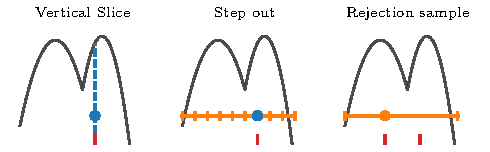
\includegraphics[width=\textwidth]{figures/slice_sampling_diagram}
    \end{columns}
\end{frame}

\begin{frame}
    \frametitle{BlackJAX Nested Slice Sampling}
    \begin{columns}
        \column{0.5\textwidth}
        \begin{block}{Core Algorithm}
            \begin{itemize}
                \item \textbf{Slice sampling} for constrained sampling
                \item Generate new live points: $\{\theta \sim \pi : \mathcal{L}(\theta) > \mathcal{L}_*\}$
                \item Vectorized operations across live points
                \item JAX transformations: \texttt{jit}, \texttt{vmap}, \texttt{grad}
            \end{itemize}
        \end{block}
        \begin{block}{GPU Advantages}
            \begin{itemize}
                \item \textbf{Parallel live points}: $n_{\text{live}} \sim 100\text{-}1000$
                \item \textbf{Vectorized slice sampling}
                \item \textbf{Batch likelihood evaluations}
                \item \textbf{Memory-efficient} on GPU
            \end{itemize}
        \end{block}
        \column{0.5\textwidth}
        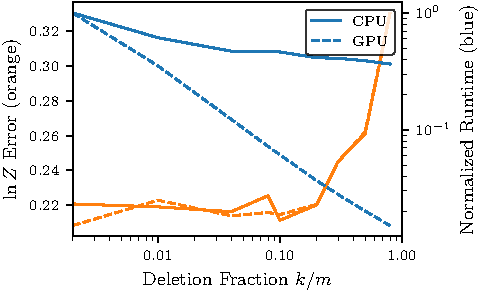
\includegraphics[width=\textwidth]{figures/scaling}
        \vspace{10pt}
        \begin{itemize}
            \item \textbf{Performance scaling}: Linear with $n_{\text{live}}$
            \item \textbf{GPU speedup}: $10\times$-$100\times$ vs CPU
            \item \textbf{Memory usage}: Constant per live point
        \end{itemize}
    \end{columns}
\end{frame}

\begin{frame}
    \frametitle{Accelerating Scientific Discovery: The Broader Impact}
    \begin{columns}
        \column{0.6\textwidth}
        \begin{block}{Connecting to Workshop Themes}
            \begin{itemize}
                \item \textbf{Experimental Design}: Nested sampling enables efficient model comparison for optimal experiment selection
                \item \textbf{Amortized Inference}: GPU vectorization amortizes computational cost across ensemble
                \item \textbf{Scientific Workflows}: BlackJAX integrates with ML pipelines (JAX ecosystem)
                \item \textbf{Diffusion Models}: Evidence computation enables model selection between generative approaches
            \end{itemize}
        \end{block}
        \begin{block}{Real-World Impact}
            \begin{itemize}
                \item \textbf{LIGO/Virgo}: Real-time gravitational wave analysis
                \item \textbf{Cosmology}: Model comparison for dark energy theories
                \item \textbf{Climate Science}: Parameter estimation in complex Earth system models
                \item \textbf{Drug Discovery}: Bayesian optimization of molecular properties
            \end{itemize}
        \end{block}
        \column{0.4\textwidth}
        \vspace{20pt}
        \begin{center}
        \textbf{The Missing Link}\\[10pt]
        \begin{itemize}
            \item Traditional MCMC: \\ \emph{Samples but no evidence}
            \item Neural approaches: \\ \emph{Fast but approximate}
            \item Nested Sampling: \\ \emph{Exact evidence + samples}
            \item GPU Acceleration: \\ \emph{Speed without approximation}
        \end{itemize}
        \end{center}
    \end{columns}
\end{frame}

\begin{frame}
    \frametitle{Performance Comparisons}
    \begin{columns}
        \column{0.5\textwidth}
        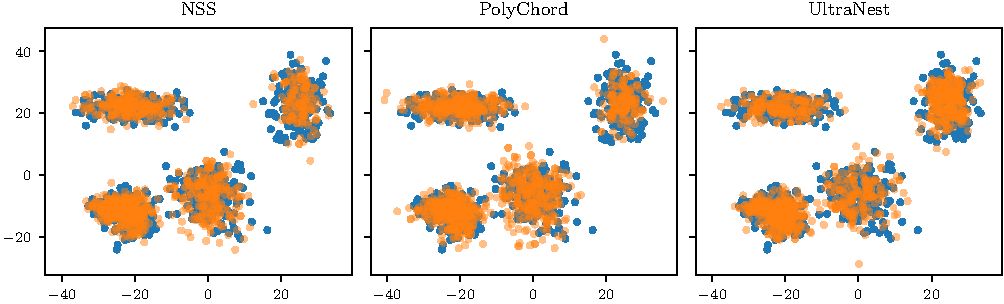
\includegraphics[width=\textwidth]{figures/pc_comparison}
        \vspace{5pt}
        \begin{itemize}
            \item Comparison with PolyChord (CPU)
            \item Same accuracy, faster convergence
            \item GPU memory efficiency
        \end{itemize}
        \column{0.5\textwidth}
        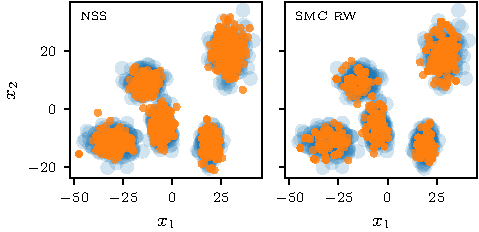
\includegraphics[width=\textwidth]{figures/mixture_gaussians_high_dim}
        \vspace{5pt}
        \begin{itemize}
            \item High-dimensional test problems
            \item Robust multimodal sampling
            \item Consistent evidence estimates
        \end{itemize}
    \end{columns}
\end{frame}

% \begin{frame}
%     \frametitle{Applications: Gravitational Wave Parameter Estimation}
%     \student{david_yallup}{David Yallup}{PDRA}
%     \begin{columns}
%         \column{0.6\textwidth}
%         \begin{itemize}
%             \item \textbf{LIGO/Virgo data analysis}:
%                 \begin{itemize}
%                     \item Binary merger parameter estimation
%                     \item 15+ dimensional parameter spaces
%                     \item Complex, multimodal posteriors
%                     \item Real-time analysis requirements
%                 \end{itemize}
%             \item \textbf{GPU advantages}:
%                 \begin{itemize}
%                     \item Parallel waveform generation
%                     \item Vectorized likelihood evaluations
%                     \item $>10\times$ speedup for parameter estimation
%                     \item Memory-efficient for long signals
%                 \end{itemize}
%             \item \textbf{Evidence computation}:
%                 \begin{itemize}
%                     \item Model comparison (GR vs modified gravity)
%                     \item Detection vs noise discrimination
%                     \item Population studies
%                 \end{itemize}
%         \end{itemize}
%         \column{0.4\textwidth}
%         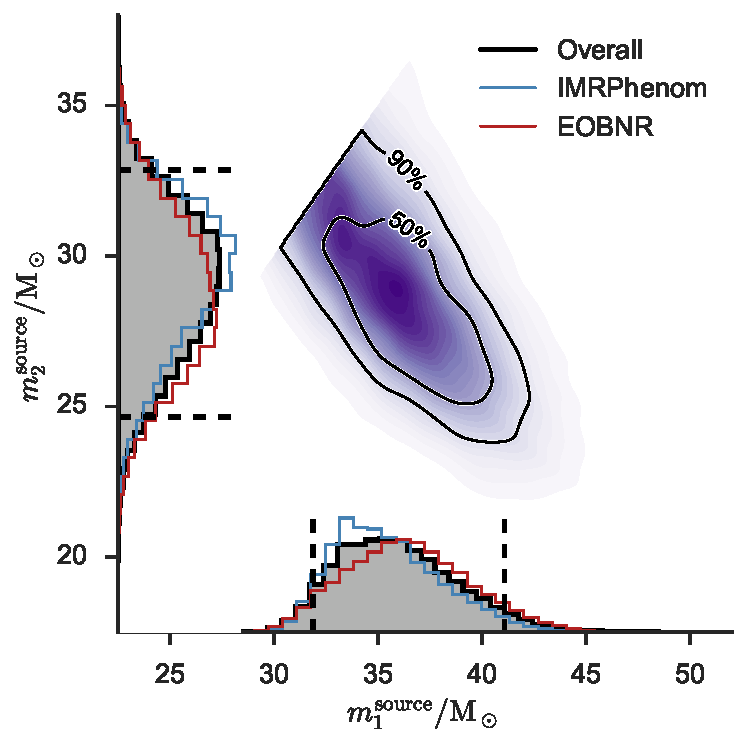
\includegraphics[width=0.49\textwidth]{figures/ligo_m1_m2}
%         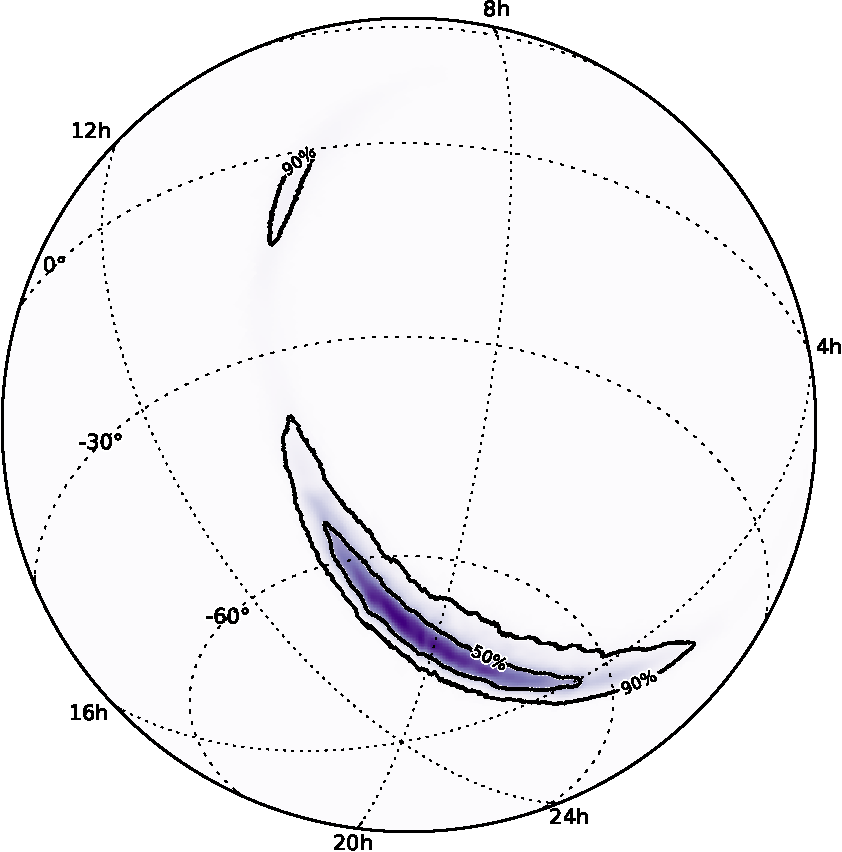
\includegraphics[width=0.49\textwidth]{figures/ligo_lambert-skymap}
%         \vspace{10pt}
%         \begin{itemize}
%             \item Mass-mass posterior
%             \item Sky localization
%             \item Real-time follow-up enabled
%         \end{itemize}
%     \end{columns}
% \end{frame}

% \begin{frame}
%     \frametitle{Applications: CMB Cosmology}
%     \student{adam_ormondroyd}{Adam Ormondroyd}{PhD}
%     \begin{columns}
%         \column{0.55\textwidth}
%         \begin{itemize}
%             \item \textbf{Cosmological parameter inference}:
%                 \begin{itemize}
%                     \item $\Lambda$CDM and extensions
%                     \item 6-20+ dimensional parameter spaces
%                     \item Non-Gaussian posteriors common
%                     \item Model comparison critical
%                 \end{itemize}
%             \item \textbf{GPU acceleration benefits}:
%                 \begin{itemize}
%                     \item Vectorized $C_\ell$ computations
%                     \item Parallel likelihood evaluations
%                     \item Large survey data volumes
%                     \item Systematic exploration of model space
%                 \end{itemize}
%             \item \textbf{Tension quantification}:
%                 \begin{itemize}
%                     \item CMB vs local universe measurements
%                     \item Evidence ratios: $\mathcal{R} = \mathcal{Z}_{AB}/(\mathcal{Z}_A \mathcal{Z}_B)$
%                     \item Suspiciousness calculations
%                 \end{itemize}
%         \end{itemize}
%         \column{0.45\textwidth}
%         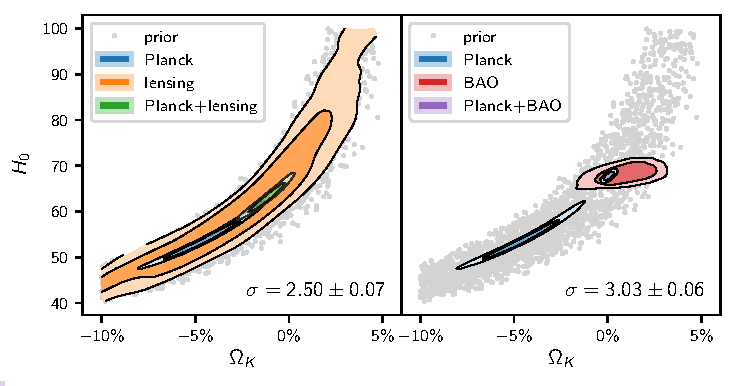
\includegraphics[width=\textwidth]{figures/omegak_H0_2}
%         \vspace{5pt}
%         \begin{itemize}
%             \item Curvature-Hubble tension
%             \item Non-Gaussian posteriors
%             \item Model comparison essential
%         \end{itemize}
%     \end{columns}
% \end{frame}

\begin{frame}
    \frametitle{The Real AI Revolution: LLMs as the Missing Piece}
    \begin{columns}
        \column{0.48\textwidth}
        \begin{block}{LLMs: The GPU Code Translator}
            \begin{itemize}
                \item \textbf{The missing piece} for porting legacy code to GPUs
                \item Automated translation: Fortran/C++ $\rightarrow$ JAX/PyTorch
                \item Handles boilerplate, vectorization patterns
                \item Bridges the gap between legacy science and modern hardware
            \end{itemize}
        \end{block}
        \begin{block}{The 80/20 Rule of Scientific Work}
            \begin{itemize}
                \item \textbf{80\% ``boring'' tasks}: Spreadsheets, forms, papers, grants, reviews, grading, code writing
                \item \textbf{20\% hard thinking}: Novel insights, experimental design, theory
                \item \textbf{AI's biggest impact}: Automating the 80\%, not the 20\%
            \end{itemize}
        \end{block}
        \column{0.48\textwidth}
        \begin{block}{Beyond Scientific Analysis}
            \begin{itemize}
                \item \textbf{Common focus}: Using LLMs for data analysis
                \item \textbf{Real transformation}: Automating scientific workflow
                \item \textbf{Already happening}:
                    \begin{itemize}
                        \item Grant writing assistance
                        \item Paper drafting and review
                        \item Code generation and debugging
                        \item Literature review automation
                    \end{itemize}
            \end{itemize}
        \end{block}
        \begin{block}{The Productivity Explosion}
            \begin{itemize}
                \item \textbf{Success story}: My group's paper production rate
                \item \textbf{New bottleneck}: \emph{``Papers generated so fast I can't review them all''}
                \item \textbf{Quality control}: Becomes the limiting factor
                \item \textbf{Focus shift}: From writing to critical thinking
            \end{itemize}
        \end{block}
    \end{columns}
\end{frame}

\begin{frame}
    \frametitle{Conclusions}
    \framesubtitle{\tthref{github.com/handley-lab/group}}
    \tikz[overlay,remember picture]
        \node[anchor=north east] (A) at ($(current page.north east)+(0,0)$) {
        
\includegraphics[width=0.09\textheight]{people/adam_ormondroyd.jpg}%
        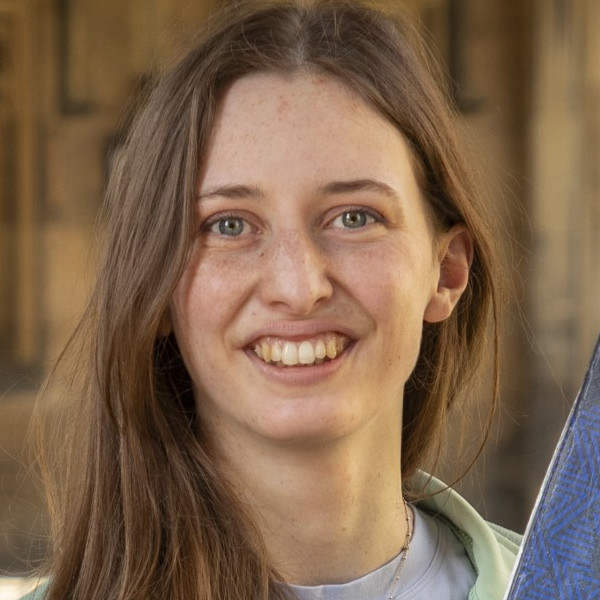
\includegraphics[width=0.09\textheight]{people/charlotte_priestley.jpg}%
        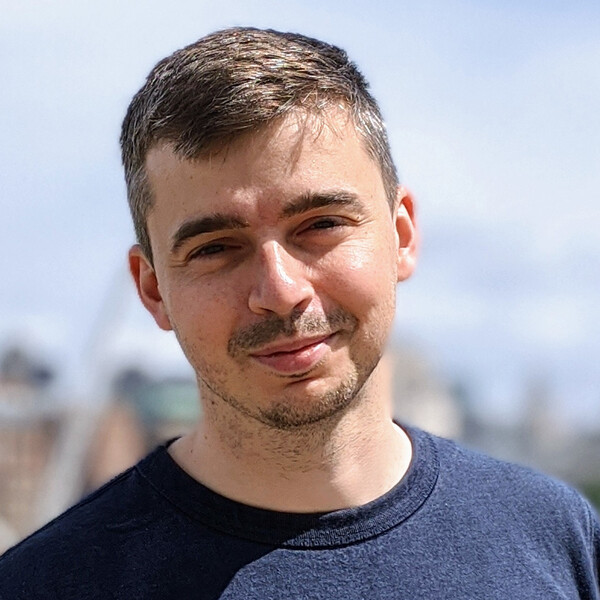
\includegraphics[width=0.09\textheight]{people/david_yallup.jpg}%
        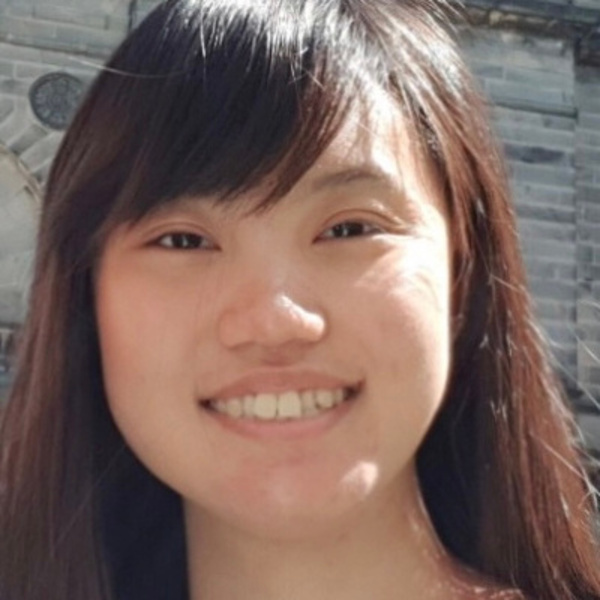
\includegraphics[width=0.09\textheight]{people/dily_ong.jpg}%
        
\includegraphics[width=0.09\textheight]{people/harry_bevins.jpg}%
        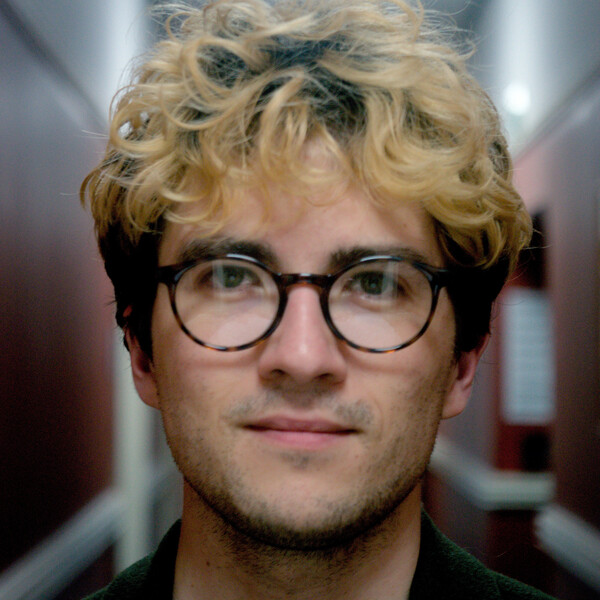
\includegraphics[width=0.09\textheight]{people/harvey_williams.jpg}%
        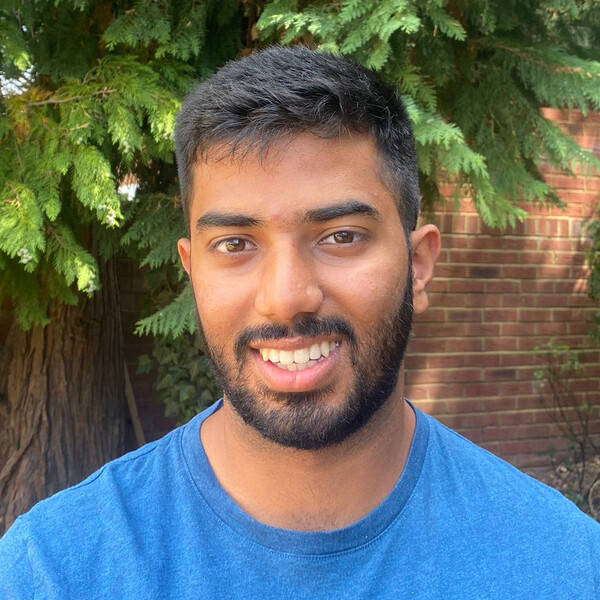
\includegraphics[width=0.09\textheight]{people/krish_nanavati.jpg}%
        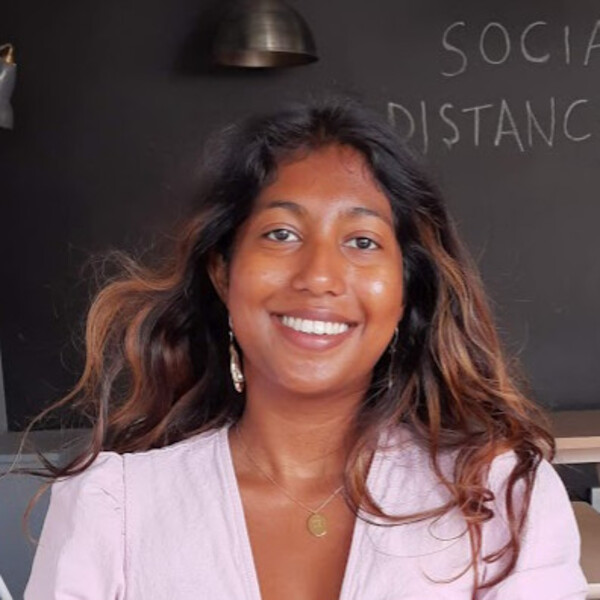
\includegraphics[width=0.09\textheight]{people/metha_prathaban.jpg}%
        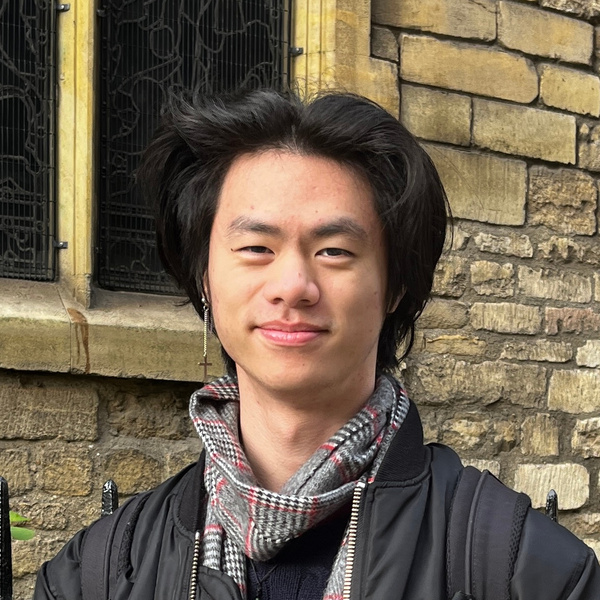
\includegraphics[width=0.09\textheight]{people/ming_yang.jpg}%
        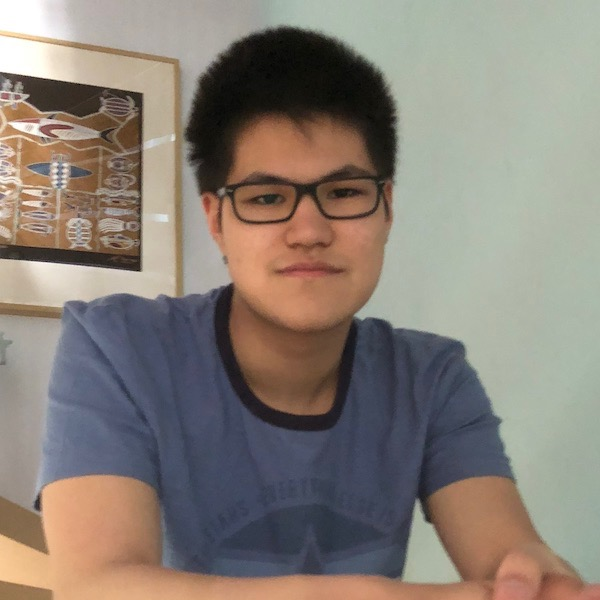
\includegraphics[width=0.09\textheight]{people/namu_kroupa.jpg}%
        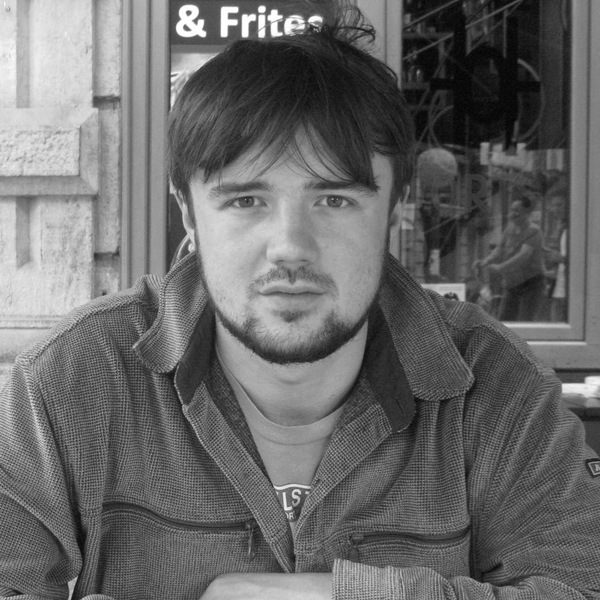
\includegraphics[width=0.09\textheight]{people/sam_leeney.jpg}%
        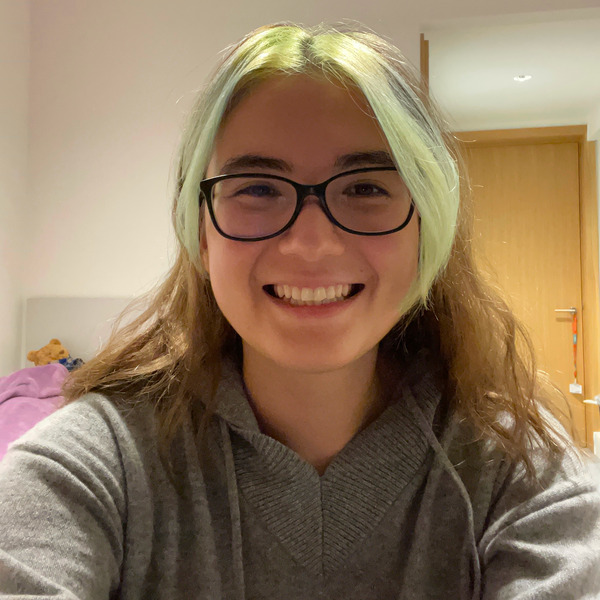
\includegraphics[width=0.09\textheight]{people/sinah_legner.jpg}%
        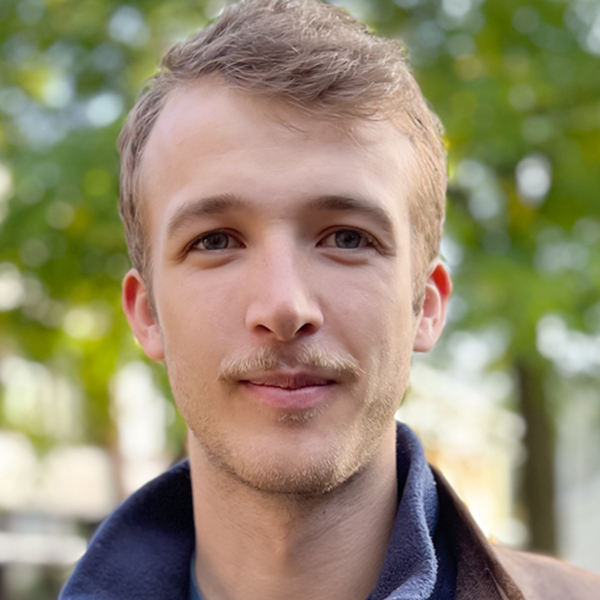
\includegraphics[width=0.09\textheight]{people/toby_lovick.jpg}%
        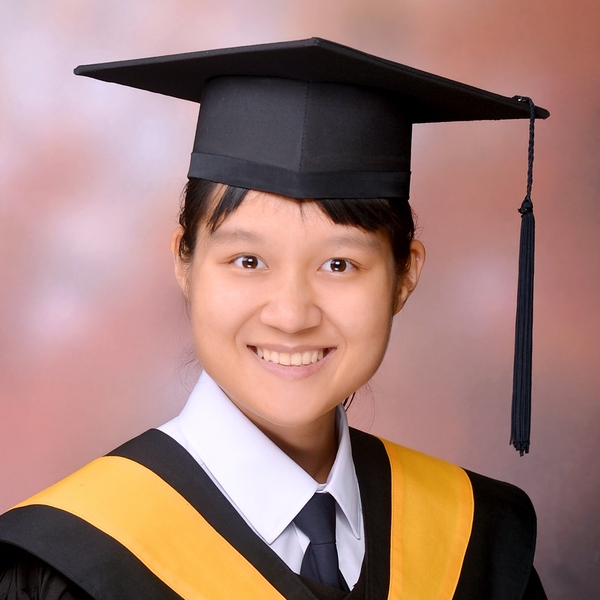
\includegraphics[width=0.09\textheight]{people/wei-ning_deng.jpg}%
        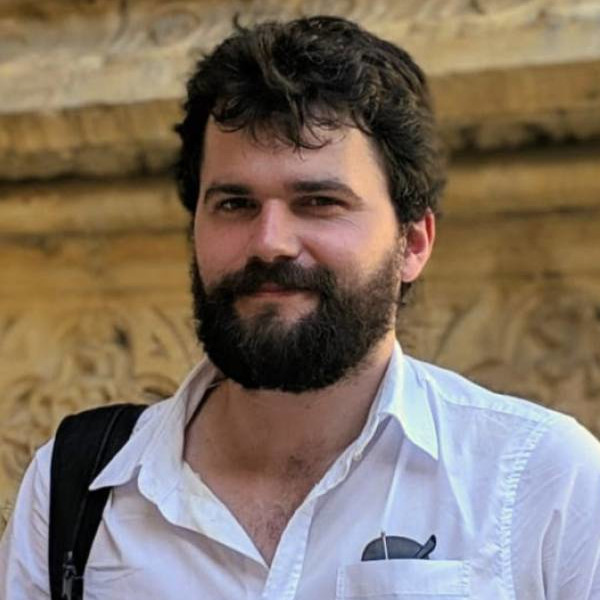
\includegraphics[width=0.09\textheight]{people/will_handley.jpg}%
        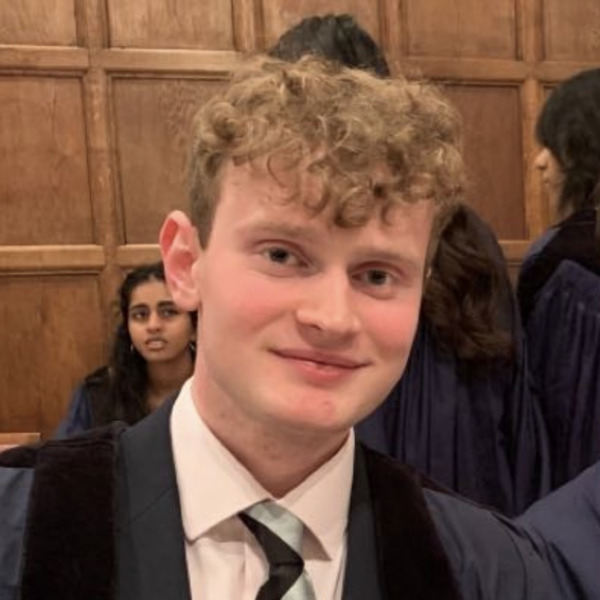
\includegraphics[width=0.09\textheight]{people/will_templeton.jpg}%
    };
\end{frame}

% Appendix
\appendix

\begin{frame}
    \frametitle{Appendix: Sequential Monte Carlo Connection}
    \begin{columns}
        \column{0.48\textwidth}
        \begin{block}{SMC Framework}
            \begin{itemize}
                \item Rigorous statistical foundation
                \item Tempered distributions: $p_t(\theta) \propto \mathcal{L}(\theta)^{\beta_t} \pi(\theta)$
                \item Nested sampling as special case of SMC
                \item Adaptive temperature schedules
            \end{itemize}
        \end{block}
        \begin{block}{Key Differences}
            \begin{itemize}
                \item \textbf{SMC}: Annealing in temperature $\beta_t$
                \item \textbf{NS}: Annealing in likelihood threshold $\mathcal{L}_*$
                \item \textbf{SMC}: Flexible inner kernels
                \item \textbf{NS}: Specialized for constrained sampling
            \end{itemize}
        \end{block}
        \column{0.48\textwidth}
        \begin{block}{BlackJAX Implementation}
            \begin{itemize}
                \item Direct comparison possible:
                    \begin{itemize}
                        \item Same GPU codebase
                        \item Identical likelihood evaluations
                        \item Fair benchmarking
                    \end{itemize}
                \item SMC with adaptive tempering
                \item Nested sampling with slice sampling
                \item Both estimate evidence $\mathcal{Z}$
            \end{itemize}
        \end{block}
        \vspace{10pt}
        \begin{center}
            \textbf{Perspective:}\\
            Statistics community: NS $\subset$ SMC\\
            Physics community: SMC $\approx$ NS variant
        \end{center}
    \end{columns}
\end{frame}

\end{document}
